\documentclass[8pt,aspectratio = 169]{beamer}

\usetheme[sectionpage=none, subsectionpage=progressbar]{metropolis}
\useoutertheme[subsection=false,footline=authortitle]{miniframes}
\setbeamertemplate{footline}[frame number]
\hypersetup{pdfpagemode=FullScreen}
\hypersetup{pdfpagelayout=SinglePage}

%-------------------------------------------------------
% INCLUDE PACKAGES
%-------------------------------------------------------

\usepackage[utf8]{inputenc}
\usepackage[english,brazil]{babel}
\usepackage[T1]{fontenc}
\usepackage{helvet}
\usepackage[num]{abntex2cite}
\citebrackets[]
\usepackage{pgfplots}
\usepackage{amsmath}
\usepackage{pdflscape}
\usepackage{afterpage}
\usepackage{capt-of}
\usepackage{booktabs}
\usepackage{array}
\usepackage{multirow}
\usepackage{longtable}
\usepackage{siunitx} 
\newcolumntype{T}[1]{S[table-format=#1]}
\newcommand\mc[1]{\multicolumn{1}{c}{#1}}
\usepackage{graphicx}
\usepackage{caption}
\usepackage{tikz} 
\usetikzlibrary{decorations.pathreplacing} % Biblioteca TikZ para as chaves ({})
\usepackage{cancel}

% Configuração das molduras ao redor das figuras e tabelas da seção 7.3
\setlength{\fboxsep}{4pt}
\setlength{\fboxrule}{0.8pt}

%-------------------------------------------------------
% DEFFINING AND REDEFINING COMMANDS
%-------------------------------------------------------
\newcommand{\chref}[2]{
  \href{#1}{{\usebeamercolor[bg]{Feather}#2}}
}

%-------------------------------------------------------
% INFORMATION IN THE TITLE PAGE
%-------------------------------------------------------
\title[] 
{ 
      \textbf{Soluções das EDOs por Séries.}
}

\subtitle[]
{
    %\textbf{Eletrônica Digital 2\\}
    Funções especiais 
}

\author[L. Silva]
{ \normalsize      
      Autores: Luiz Felipe Souza de Lima Silva}

\institute[]
{\small
      Universidade Federal do Pará (UFPA) \\
      Campus Universitário de Tucuruí \\
      Faculdade de Engenharia Elétrica \\
}

\date{2026}

%-------------------------------------------------------
% THE BODY OF THE PRESENTATION
%-------------------------------------------------------

\begin{document}

\begin{frame}[plain,noframenumbering] 
  \titlepage 
\end{frame}

\begin{frame}{Sumário de apresentação}
\tableofcontents
\end{frame}

%-------------------------------------------------------
\section{Introdução}

\section{Resoluções}

%=====================================================================================

\subsection{Questão 1}

\begin{frame}{Questão 1}

\begin{figure}[h]
    \centering
    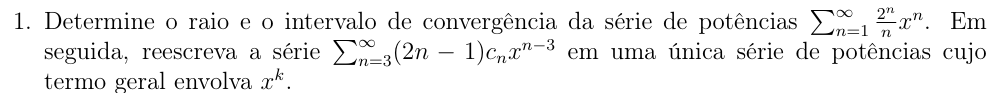
\includegraphics[width=0.9\textwidth]{q1.png}
    \label{fig:q1}
\end{figure}

\setbeamercolor{block title}{bg=structure.fg, fg=white}
\setbeamercolor{block body}{bg=structure.fg!10, fg=black}
  
  \begin{block}{Conceito chave:}
    Define-se o intervalo de convergencia aplicando a razão de teste no  coeficiente $Cn$:

\[
\text{Seja}:
\quad
\sum_{n=0}^{\infty} c_n (x - a)^n
\]

\[
\text{Aplicamos o teste da razão aos coeficientes } c_n:
\quad
L = \lim_{n \to \infty} \left| \frac{c_{n+1}}{c_n} \right|
\]

O raio será o inverso de $L$ e o intervalo de convergência por definição é $|x| < R = \frac{1}{2}$.
  \end{block}

\end{frame}


% Utilizando allowframebreaks para agrupar as resoluções em um único ponto (bolinha)
\begin{frame}[allowframebreaks]{Solução da Questão 1}

\[ 
\sum_{n=1}^{\infty} \frac{2^n}{n} x^n \qquad c_n = \frac{2^n}{n} 
\]

Portanto:
\[ 
L =  \lim_{n \to \infty} \left| \frac{c_{n+1} (x-0)^{n+1}}{c_n (x-0)^n} \right| = \lim_{n \to \infty} \left| \frac{\frac{2^{n+1}}{n+1}}{\frac{2^n}{n}} \right| 
\]

Portanto:
\[ 
L=|x| \cdot \lim_{n \to \infty} \left| \frac{2^{n+1}}{n+1} \cdot \frac{n}{2^n} \right| =  \lim_{n \to \infty} \left| \frac{2^1 \cdot n}{n+1} \right| 
\]

\[ 
\therefore L= \cdot \lim_{n \to \infty} \left| \frac{n(2)}{n(1 + \frac{1}{n})} \right| =    \lim_{n \to \infty} \left| \frac{2}{1} \right| =  2 
\]

$\therefore$ Raio de convergência $= \frac{1}{L} = \frac{1}{2}$

\framebreak % Quebra de página sem criar nova bolinha

Intervalo de convergência:
\[ 
|x| \cdot 2 < 1 \implies x < \frac{1}{2} \text{ ou } -x < \frac{1}{2} \rightarrow x > -\frac{1}{2} 
\]

Converge nesse intervalo,

Portanto:
\[ 
-\frac{1}{2} < x < \frac{1}{2} 
\]

\vspace{0.5cm}
\begin{center}
\begin{tikzpicture}
    % Reta real
    \draw[<-] (-3,0) -- (3,0);
    \node at (-3.2, 0) {$R$};
    
    % Linha ondulada (intervalo de convergência)
    \draw[thick, decorate, decoration={snake, amplitude=0.5mm, segment length=3mm}] (-2,0) -- (2,0);
    
    % Pontos abertos
    \draw[fill=white, thick] (-2,0) circle (0.1) node[below=0.2cm] {$-\frac{1}{2}$};
    \draw[fill=white, thick] (2,0) circle (0.1) node[below=0.2cm] {$\frac{1}{2}$};
\end{tikzpicture}
\end{center}
\vspace{0.5cm}

\framebreak % Quebra de página sem criar nova bolinha

reduzindo : \[
\sum_{n=3}^{\infty} (2n - 1)c_n x^{n-3}
\]
\[
\sum_{n=3}^{\infty} (2n - 1) c_n x^{n-3}
\quad \text{com} \quad k = n - 3 \Rightarrow n = k + 3
\]

\[
\text{Portanto:} \quad
\sum_{k=0}^{\infty} [2(k+3) - 1] c_{k+3} x^k
= \sum_{k=0}^{\infty} (2k + 5) c_{k+3} x^k
\]

\end{frame}

%=====================================================================================

\subsection{Questão 2}

\begin{frame}{Questão 2}

\begin{figure}[h]
    \centering
    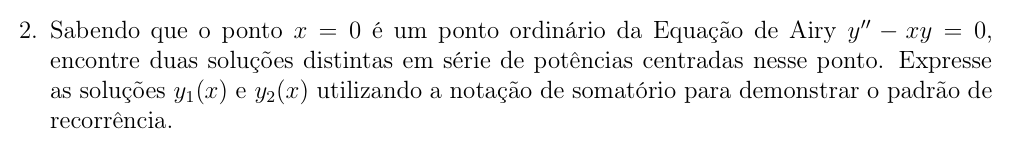
\includegraphics[width=0.9\textwidth]{q2.png}
    \label{fig:q2}
\end{figure}

\setbeamercolor{block title}{bg=structure.fg, fg=white}
\setbeamercolor{block body}{bg=structure.fg!10, fg=black}

 \begin{block}{Conceito chave:}
Devido o ponto $x=0$ ser um ponto ordinário, ou seja, regular, podemos admitir a seguinte hipótese de solução:
\\
\[ y(x) = \sum_{n=0}^{\infty} C_n x^n ;\]
    
\end{block}
    
\end{frame}

\begin{frame}[allowframebreaks]{Solução da Questão 2}
\small 

Portanto:
\[ 
y(x) = \sum_{n=0}^{\infty} C_n x^n ; \quad 
y'(x) = \sum_{n=1}^{\infty} C_n (n) x^{n-1} ; \quad 
y''(x) = \sum_{n=2}^{\infty} C_n (n)(n-1) x^{n-2} 
\]

\noindent Substituindo em \[ y'' - xy = 0 \]:
\begin{align*}
    \sum_{n=2}^{\infty} C_n (n)(n-1) x^{n-2} - x \sum_{n=0}^{\infty} C_n x^n &= 0 \\[1ex]
    \therefore\sum_{n=2}^{\infty} C_n (n)(n-1) x^{n-2} - \sum_{n=0}^{\infty} C_n x^{n+1} &= 0 
\end{align*}

\begin{align*}
    \therefore[C_2(2)(1) + C_3(3)(2)x +\dots] - [C_0 x + C_1 x^2 + C_2 x^3 +\dots] &= 0 \\[1ex]
    C_2 \cdot 2 + \sum_{n=3}^{\infty} C_n (n)(n-1) x^{n-2} - \sum_{n=0}^{\infty} C_n x^{n+1} &= 0 
\end{align*}

\framebreak % Quebra

\noindent logo:
\[ C_2 \cdot 2 = 0 \rightarrow \boxed{C_2 = 0} \]
Mudança de variáveis da soma
\noindent:
\[ \sum_{n=3}^{\infty} C_n (n)(n-1) x^{n-2} - \sum_{n=0}^{\infty} C_n x^{n+1} = 0 ; \]

\begin{center}
    \begin{tabular}{cc}
        $n=3$ & $n=0$ \\
        $K = n - 2 \rightarrow n = K + 2$ & $K = n + 1 \rightarrow n = K - 1$
    \end{tabular}
\end{center}

\noindent logo:
\[ \sum_{K=1}^{\infty} C_{K+2} (K+2)(K+1) x^K - \sum_{K=1}^{\infty} C_{K-1} x^K = 0  \]

\noindent Portanto:
\[ \sum_{K=1}^{\infty} x^K [ C_{K+2} (K+2)(K+1) - C_{K-1} ] = 0 ;\]

\framebreak % Quebra

A partir de:
\[ \sum_{K=1}^{\infty} x^K [ C_{K+2} (K+2)(K+1) - C_{K-1} ] = 0 ;\]

Teremos
\noindent :
\[ C_{K+2} (K+2)(K+1) - C_{K-1} = 0 \]

\noindent A série inicia em $K=1$, portanto teremos:

\vspace{0.3cm}
\noindent P/ $K=1$:
\[ C_3 (3)(2) - C_0 = 0 \rightarrow C_3 = \frac{C_0}{6} = \frac{C_0}{3!} \]

\noindent P/ $K=2$:
\[ C_4 (4)(3) - C_1 = 0 \therefore C_4 = \frac{C_1}{4 \cdot 3} \]

\noindent P/ $K=3$:
\[ C_5 (5)(4) - C_2 = 0  \rightarrow C_5 = 0 \]

\noindent P/ $K=4$:
\[ C_6 (6)(5) - C_3 \rightarrow C_6 = \frac{C_3}{6 \cdot 5} = \frac{C_0}{3 \cdot 2} \cdot \frac{1}{6 \cdot 5} \]

\noindent P/ $K=5$:
\[ C_7 (7)(6) - C_4 \therefore C_7 = \frac{C_1}{4 \cdot 3} \cdot \frac{1}{7 \cdot 6} \]

\noindent P/ $K=6$:
\[ C_8 (8)(7) - {C_5}  = 0\rightarrow C_8 = 0 \]

\framebreak % Quebra

\noindent Portanto, teremos:

\[ y(x) = \sum_{n=0}^{\infty} C_n x^n = C_0 + C_1 x + C_2 x^2 + C_3 x^3 \dots \]

\begin{align*}
    y(x) = & C_0 + C_1 x + \cancel{C_2 x^2}^0 + \frac{C_0}{3!} x^3 + \frac{C_1}{4 \cdot 3} x^4 + \cancel{C_5 x^5}^0 \\
    & + \frac{C_0}{3 \cdot 2 \cdot 6 \cdot 5} x^6 + \frac{C_1}{4 \cdot 3 \cdot 7 \cdot 6} x^7 + \cancel{C_8 x^8}^0 \dots
\end{align*}

\begin{center}
    $\displaystyle \therefore y(x) = C_0 \left( 1 + \frac{x^3}{3!} + \frac{x^6}{3 \cdot 2 \cdot 6 \cdot 5} \dots \right) + C_1 \left( x + \frac{x^4}{4 \cdot 3} + \frac{x^7}{4 \cdot 3 \cdot 7 \cdot 6} + \dots \right);$    
\end{center}

\end{frame}

%=====================================================================================

\subsection{Questão 3}

\begin{frame}{Questão 3}

\begin{figure}[h]
    \centering
    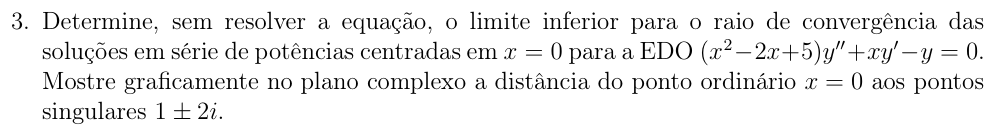
\includegraphics[width=0.9\textwidth]{q3.png}
    \label{fig:q3}
\end{figure}

\setbeamercolor{block title}{bg=structure.fg, fg=white}
\setbeamercolor{block body}{bg=structure.fg!10, fg=black}

\begin{block}{Conceito chave}
    Para determinar o Limite inferior para o raio de Convergência da série, devemos verificar a distância do ponto de singularidade mais próximo até o centro da Série.
\end{block}
    
\end{frame}

\begin{frame}[allowframebreaks]{Solução da Questão 3}

\noindent\underline{Portanto:}
\[ (x^2 - 2x + 5)y'' + xy' - y = 0 ; \quad \rightarrow \text{centrado em } x=0 . \]

\begin{itemize}
    \item temos que:
\end{itemize}
\[ (1+2j) \text{ e } (1-2j) \text{ são pontos singulares da série.} \]

\vspace{0.5cm}


\end{frame}
\begin{frame}[allowframebreaks]{Solução da Questão 3}

\begin{minipage}{0.5\textwidth}
\begin{center}
\begin{tikzpicture}
    % Eixos
    \draw[->] (-1,0) -- (3,0) node[right] {$Re$};
    \draw[->] (0,-3) -- (0,3) node[above] {$Im$};

    % Origem e marcações
    \node[below left] at (0,0) {$0$};
    \draw (1,0.1) -- (1,-0.1) node[below] {$1$};
    \draw (0.1,2) -- (-0.1,2) node[left] {$2$};
    \draw (0.1,-2) -- (-0.1,-2) node[left] {$-2$};

    % Pontos singulares
    \filldraw (1,2) circle (1.5pt) node[right] {$P(1+2j)$};
    \filldraw (1,-2) circle (1.5pt) node[right] {$(1-2j)$};

    % Distância r
    \draw (0,0) -- (1,2) node[midway, above left] {$r$};
    \draw (0,0) -- (1,-2) node[midway, below left] {$r$};
    
    % Linhas tracejadas
    \draw[dashed] (1,0) -- (1,2);
    \draw[dashed] (1,0) -- (1,-2);
\end{tikzpicture}
\end{center}
\end{minipage}%
\begin{minipage}{0.5\textwidth}
    \underline{Portanto:}
    \[ dOP = |1+2j| = \sqrt{5} \]
    \noindent Portanto, o limite inferior do raio de convergência é $\sqrt{5} ;$
\end{minipage}


    
\end{frame}
%=====================================================================================

\subsection{Questão 4}

\begin{frame}{Questão 4}
\begin{figure}[h]
     \centering
    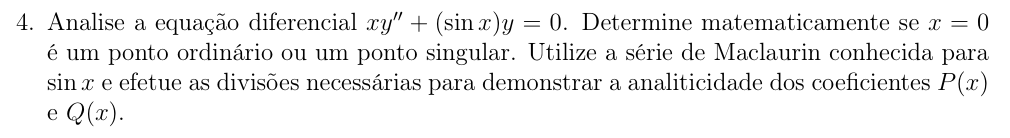
\includegraphics[width=0.9\textwidth]{q4.png}
    \label{fig:q4}
\end{figure}

\setbeamercolor{block title}{bg=structure.fg, fg=white}
\setbeamercolor{block body}{bg=structure.fg!10, fg=black}

\end{frame}

\begin{frame}[allowframebreaks]{Solução da Questão 4}
    
    \textbf{1ª Solução:}
    
    \[ xy'' + \text{sen}(x)y = 0 \quad \left(\frac{1}{x}\right) \]
    \[ y'' + \frac{\text{sen}(x)}{x} y = 0 \]
    
    Para ângulos muito pequenos, podemos usar a aproximação $\text{sen}(x) \simeq x$.
    
    Portanto, para $x \to 0$:
    \[ y'' + \frac{x}{x}y = 0 \longrightarrow \boxed{y'' + y = 0} \]
    
    \begin{itemize}
        \item Analítica em $x=0$.
    \end{itemize}

    \framebreak % Quebra
    
    \textbf{2ª Solução:}
    
    \[ y'' + \underbrace{\left( \frac{\text{sen}(x)}{x} \right)}_{\text{Expansão de Taylor em } x=0} y = 0 \]
    
    Temos que a expansão para $\text{sen}(x)$ é:
    \[ \text{sen}(x) = \sum_{n=0}^{\infty} \frac{\text{sen}^{(n)}(0)}{n!} x^n = x - \frac{x^3}{3!} + \frac{x^5}{5!} - \dots = \sum_{n=0}^{\infty} \frac{(-1)^n x^{2n+1}}{(2n+1)!} \]
    
    Sendo $P(x) = \frac{\text{sen}(x)}{x}$, substituímos a série:
    \begin{align*}
        P(x) &= \frac{1}{x} \sum_{n=0}^{\infty} \frac{(-1)^n x^{2n+1}}{(2n+1)!} \\[1ex]
        P(x) &= \frac{1}{x} \left( x - \frac{x^3}{3!} + \frac{x^5}{5!} - \frac{x^7}{7!} + \dots \right) \\[1ex]
        P(x) &= 1 - \frac{x^2}{3!} + \frac{x^4}{5!} - \frac{x^6}{7!} + \dots 
    \end{align*}
    
    \framebreak % Quebra
    
    \setbeamercolor{block title}{bg=structure.fg, fg=white}
    \setbeamercolor{block body}{bg=structure.fg!10, fg=black}

    \begin{block}{Conclusão}
        \[ \therefore P(x) = \sum_{n=0}^{\infty} \frac{(-1)^n x^{2n}}{(2n+1)!} \quad \longrightarrow \quad \text{Converge em todo } x \in \mathbb{R}. \]
    \end{block}
    
\end{frame}

\section{Conclusão}

\end{document}